% ==================================================
% 4.3 動態導航與避障比較
% ==================================================
\section{動態導航與避障比較}
\label{sec:dynamic_navigation_comparison}

移動機械臂在接近操作區域前，需先通過固定障礙與動態物件交會的空間。
本節以底盤導航控制鏈為評估範圍，
比較本研究導航配置、Nav2 MPPI 與 Regulated Pure Pursuit（RPP）
在相同場景與共同起終點下的到達、淨空及時間表現。
另透過控制屏障函數與原始雷射防護的消融比較，
分析控制求解與命令執行兩個層次對避障結果的影響。
底盤與手臂同時運動的追蹤表現則於第 4.4 節分析。

% ==================================================
% 4.3.1 動態障礙場景與測試配置
% ==================================================
\subsection{動態障礙場景與測試配置}
\label{subsec:dynamic_navigation_scenario_setup}

導航比較於 Gazebo Harmonic 建立的室內場景進行，
場景範圍約為 $20\times20$ m，
配置分隔牆、已知靜態障礙、未加入先驗地圖的靜態障礙，
以及沿設定路段往返的動態物件。
\cref{fig:ch4_dynamic_navigation_scene}呈現平面配置與障礙運動路段。
分隔牆形成不同方向的通行開口，
靜態障礙限制可用空間，
動態物件則在機器人穿越場景時形成交會需求。

\begin{figure}[htbp]
    \centering
    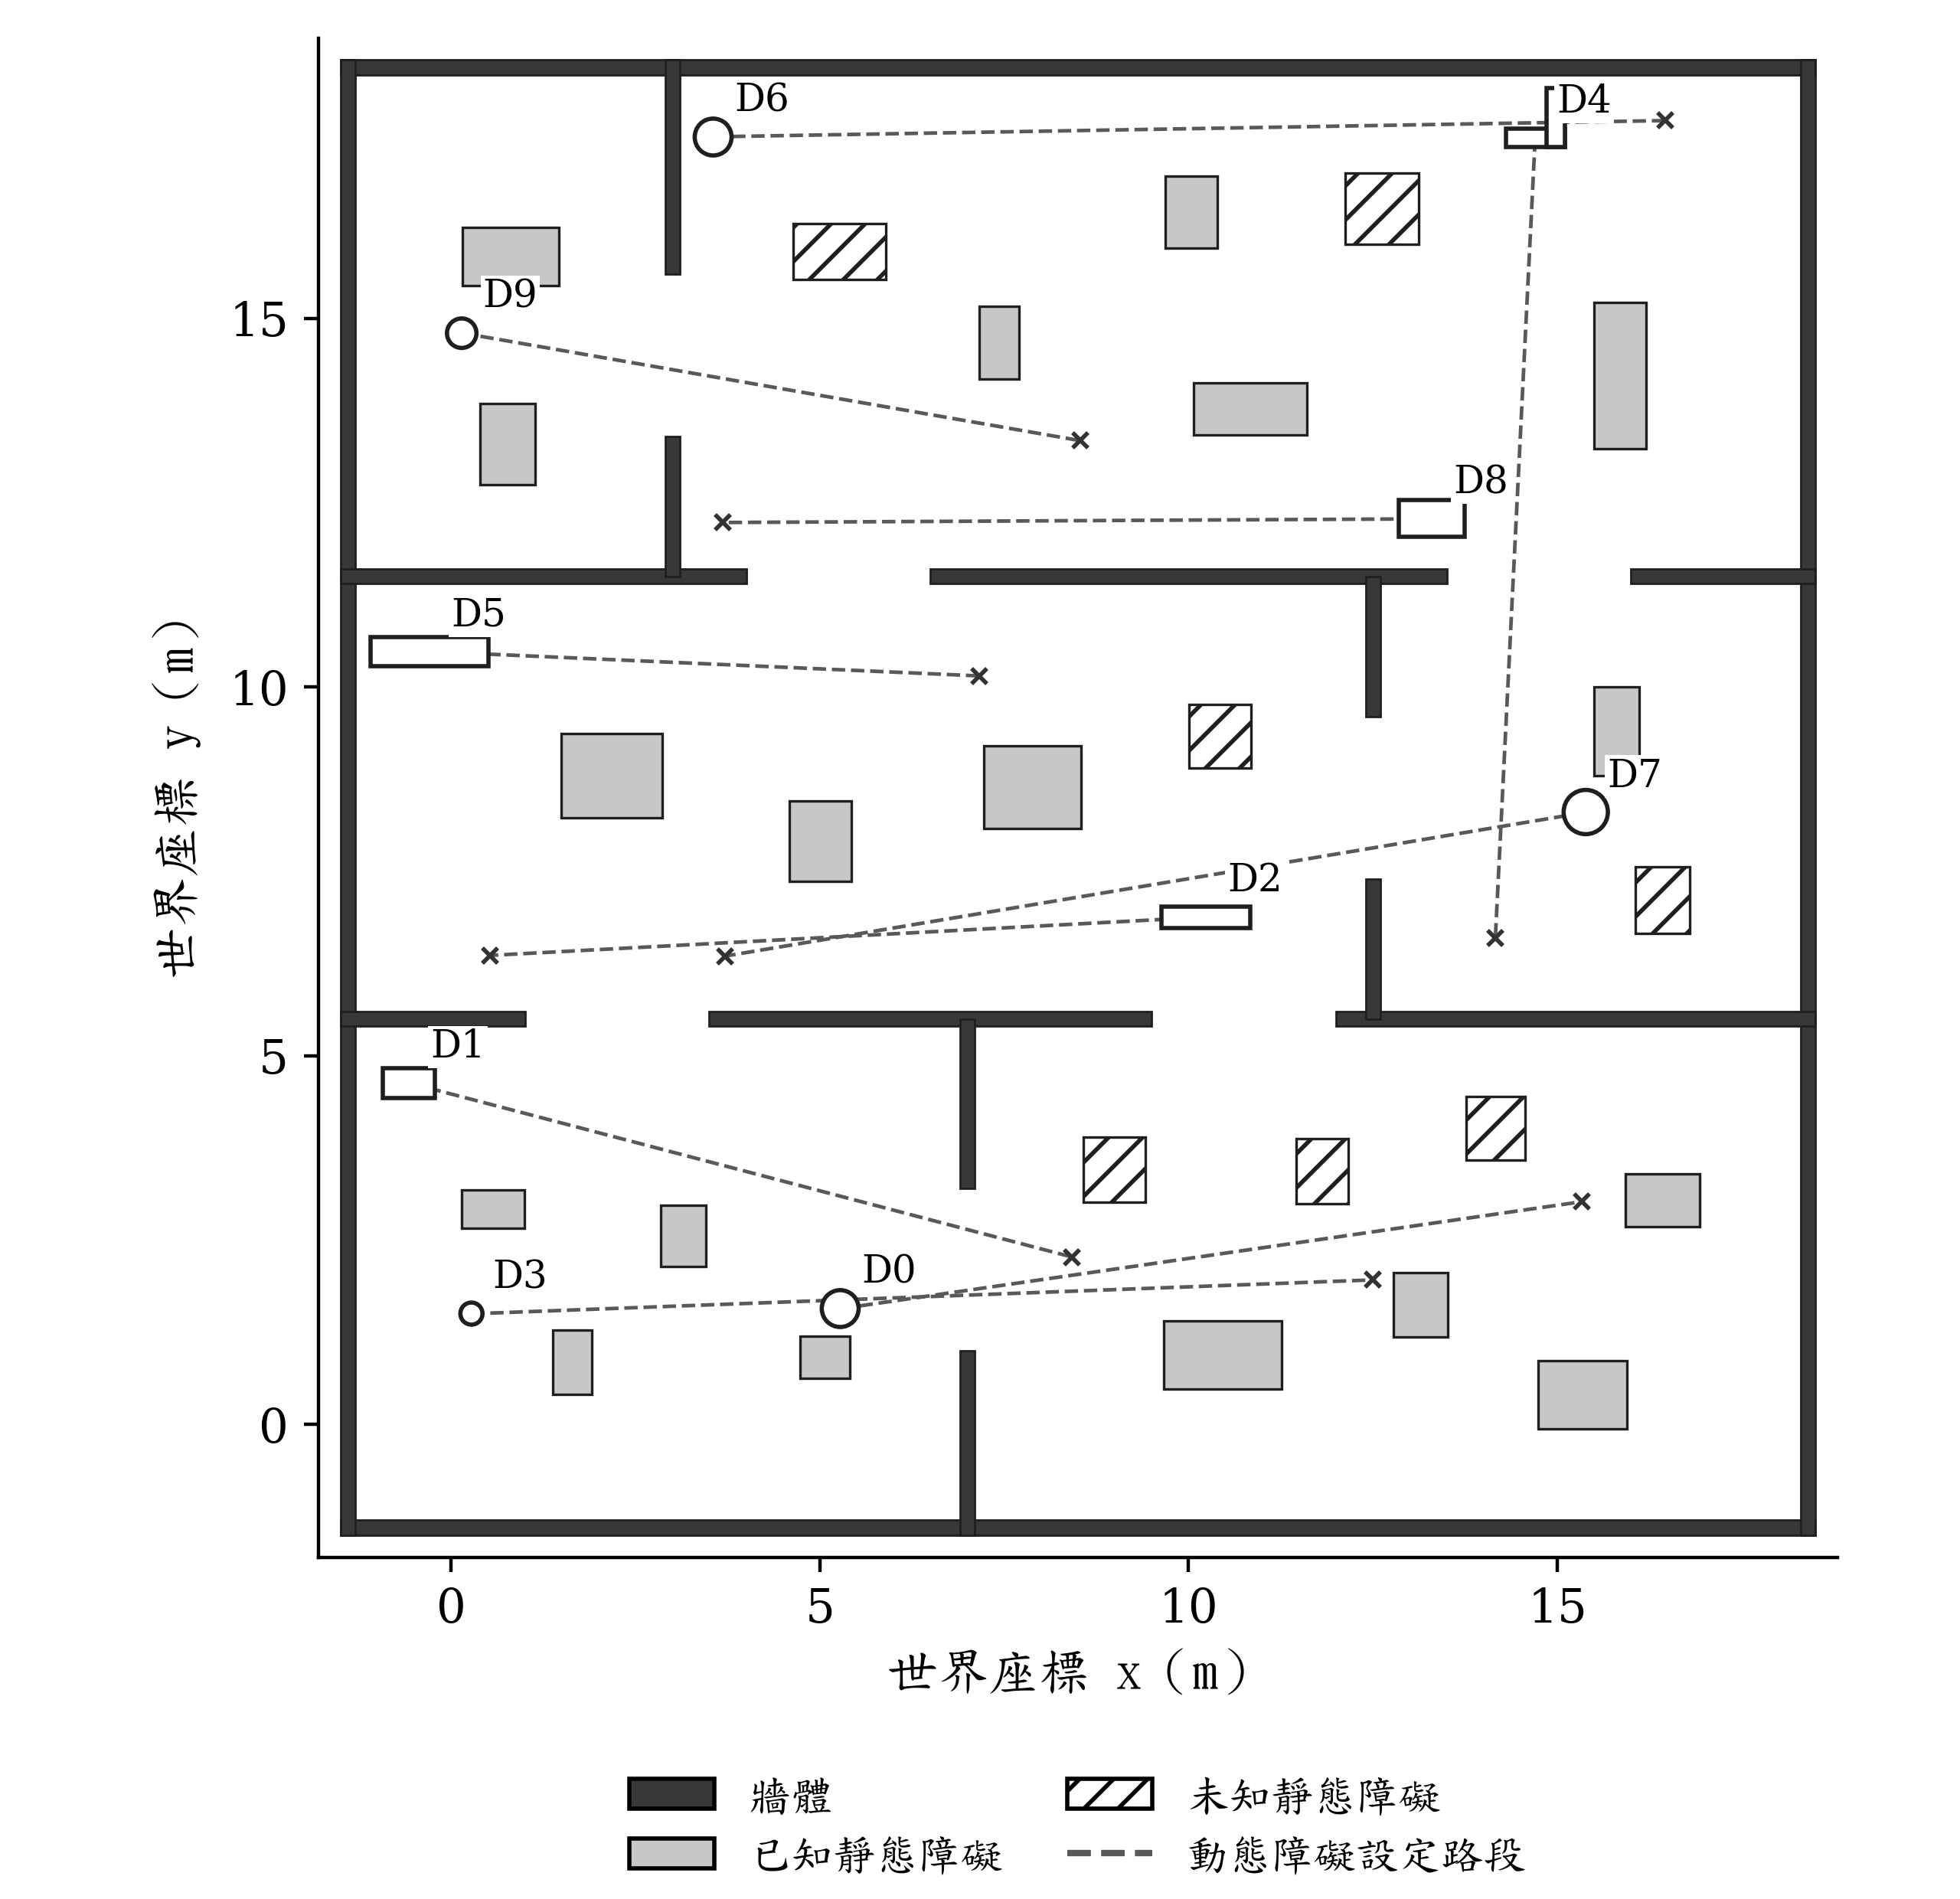
\includegraphics[width=0.92\textwidth]{figsrc/ch04/dynamic_navigation_scene.png}
    \caption{動態導航比較場景之平面配置。
    深色區域為牆體，灰色區域為已知靜態障礙，斜線區域為未知靜態障礙；
    D0--D9 表示動態物件，虛線為設定的往返路段，叉號標示另一端點。}
    \label{fig:ch4_dynamic_navigation_scene}
\end{figure}

動態場景包含十個不同外形的物件，
涵蓋圓柱、矩形與複合外形，設定移動速度介於 $0.10$--$0.14$ m/s。
各方法共用起終點清單、場景幾何及障礙運動設定，
實際交會時機則隨機器人的行進速度與避讓行為改變。
控制器由雷射與各自的感知、代價地圖或追蹤模組取得環境資訊；
模擬器回報的障礙位置另用於離線幾何評估。

本研究導航配置以 SE(2) GMPC 追蹤全域路徑，
於預測時域加入 CBF 限制，
並在命令平滑後以原始雷射防護核對近距離回波。
本組比較固定採用此導航配置，局部側移候選調整關閉。
MPPI 採用 Nav2 的全向運動模型，
以取樣控制序列及軌跡成本更新輸入\cite{nav2mppijazzy}。
RPP 則依路徑前視點與曲率調節前進速度\cite{macenski2023rpp}，
其控制命令包含前進與偏航，側向速度維持為零。

主要條件如\cref{tab:ch4_navigation_settings}所示。
三種方法在可用運動軸上使用相同的執行端速度與命令變化上限，
內部預測時域、取樣方式及成本設定則依各方法配置保留。
MPPI 的內部縱向負加速度界為 $-1.5$ m/s$^2$，
與執行端平滑器的減速限制分別設定。
因此，結果用於比較各導航控制鏈於本全向底盤上的整體表現，
其差異同時包含控制形式與可使用的運動方向。

\begin{table}[htbp]
    \centering
    \caption{動態導航比較之主要設定}
    \label{tab:ch4_navigation_settings}
    \begingroup
    \small
    \renewcommand{\arraystretch}{1.2}
    \begin{tabular}{p{0.31\textwidth} p{0.59\textwidth}}
        \hline
        項目 & 設定 \\
        \hline
        模擬平台與場景 & Gazebo Harmonic，約 $20\times20$ m \\
        動態障礙 & 十個物件，設定速度 $0.10$--$0.14$ m/s \\
        底盤平面外形 & 半徑 $0.30$ m 的圓盤 \\
        控制更新頻率 & $20$ Hz \\
        平移速度上限 & 各可用軸 $0.2775$ m/s；RPP 的 $v_y^B=0$ \\
        偏航速度上限 & $1.1327$ rad/s \\
        執行端命令變化上限
        & 平移 $6.25$ m/s$^2$、偏航 $25.51$ rad/s$^2$ \\
        GMPC 預測時域 & $20$ 步，步長 $0.05$ s，共 $1.0$ s \\
        MPPI 預測與取樣 & $56$ 步，步長 $0.05$ s，共 $2.8$ s；取樣數 $2000$ \\
        到達位置門檻 & 至目標的平面距離小於 $0.30$ m \\
        記錄時間上限 & 牆鐘時間 $250$ s \\
        \hline
    \end{tabular}
    \endgroup
\end{table}

到達結果採用已保存的控制端到達事件與位姿重建判定。
本節到達時間沿用 rosbag 記錄的接收時間戳計算，
與住宅整合任務的模擬時間分別呈現。
淨空統計由首筆全域路徑開始，
至位姿首次進入到達範圍為止；尚未進入時則計算至量測結束。
幾何評估使用底盤與動態物件的模擬位姿，
配合該組資料的靜態距離場及障礙外形近似，
取得每條路線的最小淨空。
複合動態外形於此統計中以主要矩形區塊近似，
幾何重疊結果依此平面評估範圍解讀。

令 $\hat d_r(t)$ 為第 $r$ 條路線在上述評估方式下的淨空，
定義路線最小淨空與幾何重疊指標為
\begin{equation}
    d_{\min,r}=\min_{t\in\mathcal T_r}\hat d_r(t),
    \qquad
    C_r=\mathbb I(d_{\min,r}<0),
    \label{eq:ch4_navigation_overlap_indicator}
\end{equation}
其中 $\mathcal T_r$ 為該路線的評估區間。
當 $C_r=1$ 時，表示評估外形曾出現負淨空。
同一路線內即使重複出現多個負淨空區間，
在重疊路線數中仍只計一次，
以區分路線層級的結果與反覆接近障礙所形成的事件次數。

% ==================================================
% 4.3.2 不同導航方法之性能比較
% ==================================================
\subsection{不同導航方法之性能比較}
\label{subsec:navigation_method_performance}

到達比較採用三種方法皆保有導航結果的 $83$ 條共同路線。
淨空比較另要求三種方法均具有有限且有效的淨空值，
因此使用其中資料完整的 $82$ 條路線；
缺少淨空值的路線仍保留於到達統計。
各方法的到達時間則由其已到達路線計算中位數，
使到達情形、幾何間距與時間各自對應明確的資料集合。

比較結果如\cref{tab:ch4_navigation_method_results}所示。
本研究導航配置完成全部 $83$ 條共同路線，
MPPI 與 RPP 分別到達 $64$ 與 $60$ 條。
在共同淨空集合中，三者的幾何重疊路線數依序為 $1$、$6$ 與 $30$，
每條路線最小淨空的中位數則約為 $0.175$、$0.120$ 與 $0.060$ m。
本研究導航配置在此集合中保留較大的典型間距，
並同時維持較完整的目標到達表現。

\begin{table}[htbp]
    \centering
    \caption{共同路線下之導航方法比較}
    \label{tab:ch4_navigation_method_results}
    \begingroup
    \small
    \setlength{\tabcolsep}{4pt}
    \renewcommand{\arraystretch}{1.25}
    \begin{tabular}{l c c c c}
        \hline
        方法
        & \shortstack{到達路線\\（共 $83$ 條）}
        & \shortstack{重疊路線\\（共 $82$ 條）}
        & \shortstack{最小淨空\\中位數（m）}
        & \shortstack{到達時間\\中位數（s）} \\
        \hline
        本研究導航 & $83$ & $1$  & $0.175$ & $102.6$ \\
        MPPI       & $64$ & $6$  & $0.120$ & $48.6$  \\
        RPP        & $60$ & $30$ & $0.060$ & $73.9$  \\
        \hline
    \end{tabular}
    \endgroup
\end{table}

\cref{fig:ch4_navigation_method_comparison}(a)同時呈現到達與未到達路線，
(b)則以每條路線最小淨空的經驗累積分布比較間距。
對相同淨空門檻，累積比例表示最小淨空不大於該值的路線比例。
本研究導航配置的分布主要位於正淨空區域，
MPPI 與 RPP 則包含較多低淨空或負淨空路線。
其中本研究導航配置的最差估計淨空約為 $-0.0012$ m，
對應一次接近幾何邊界的輕微重疊。

\begin{figure}[htbp]
    \centering
    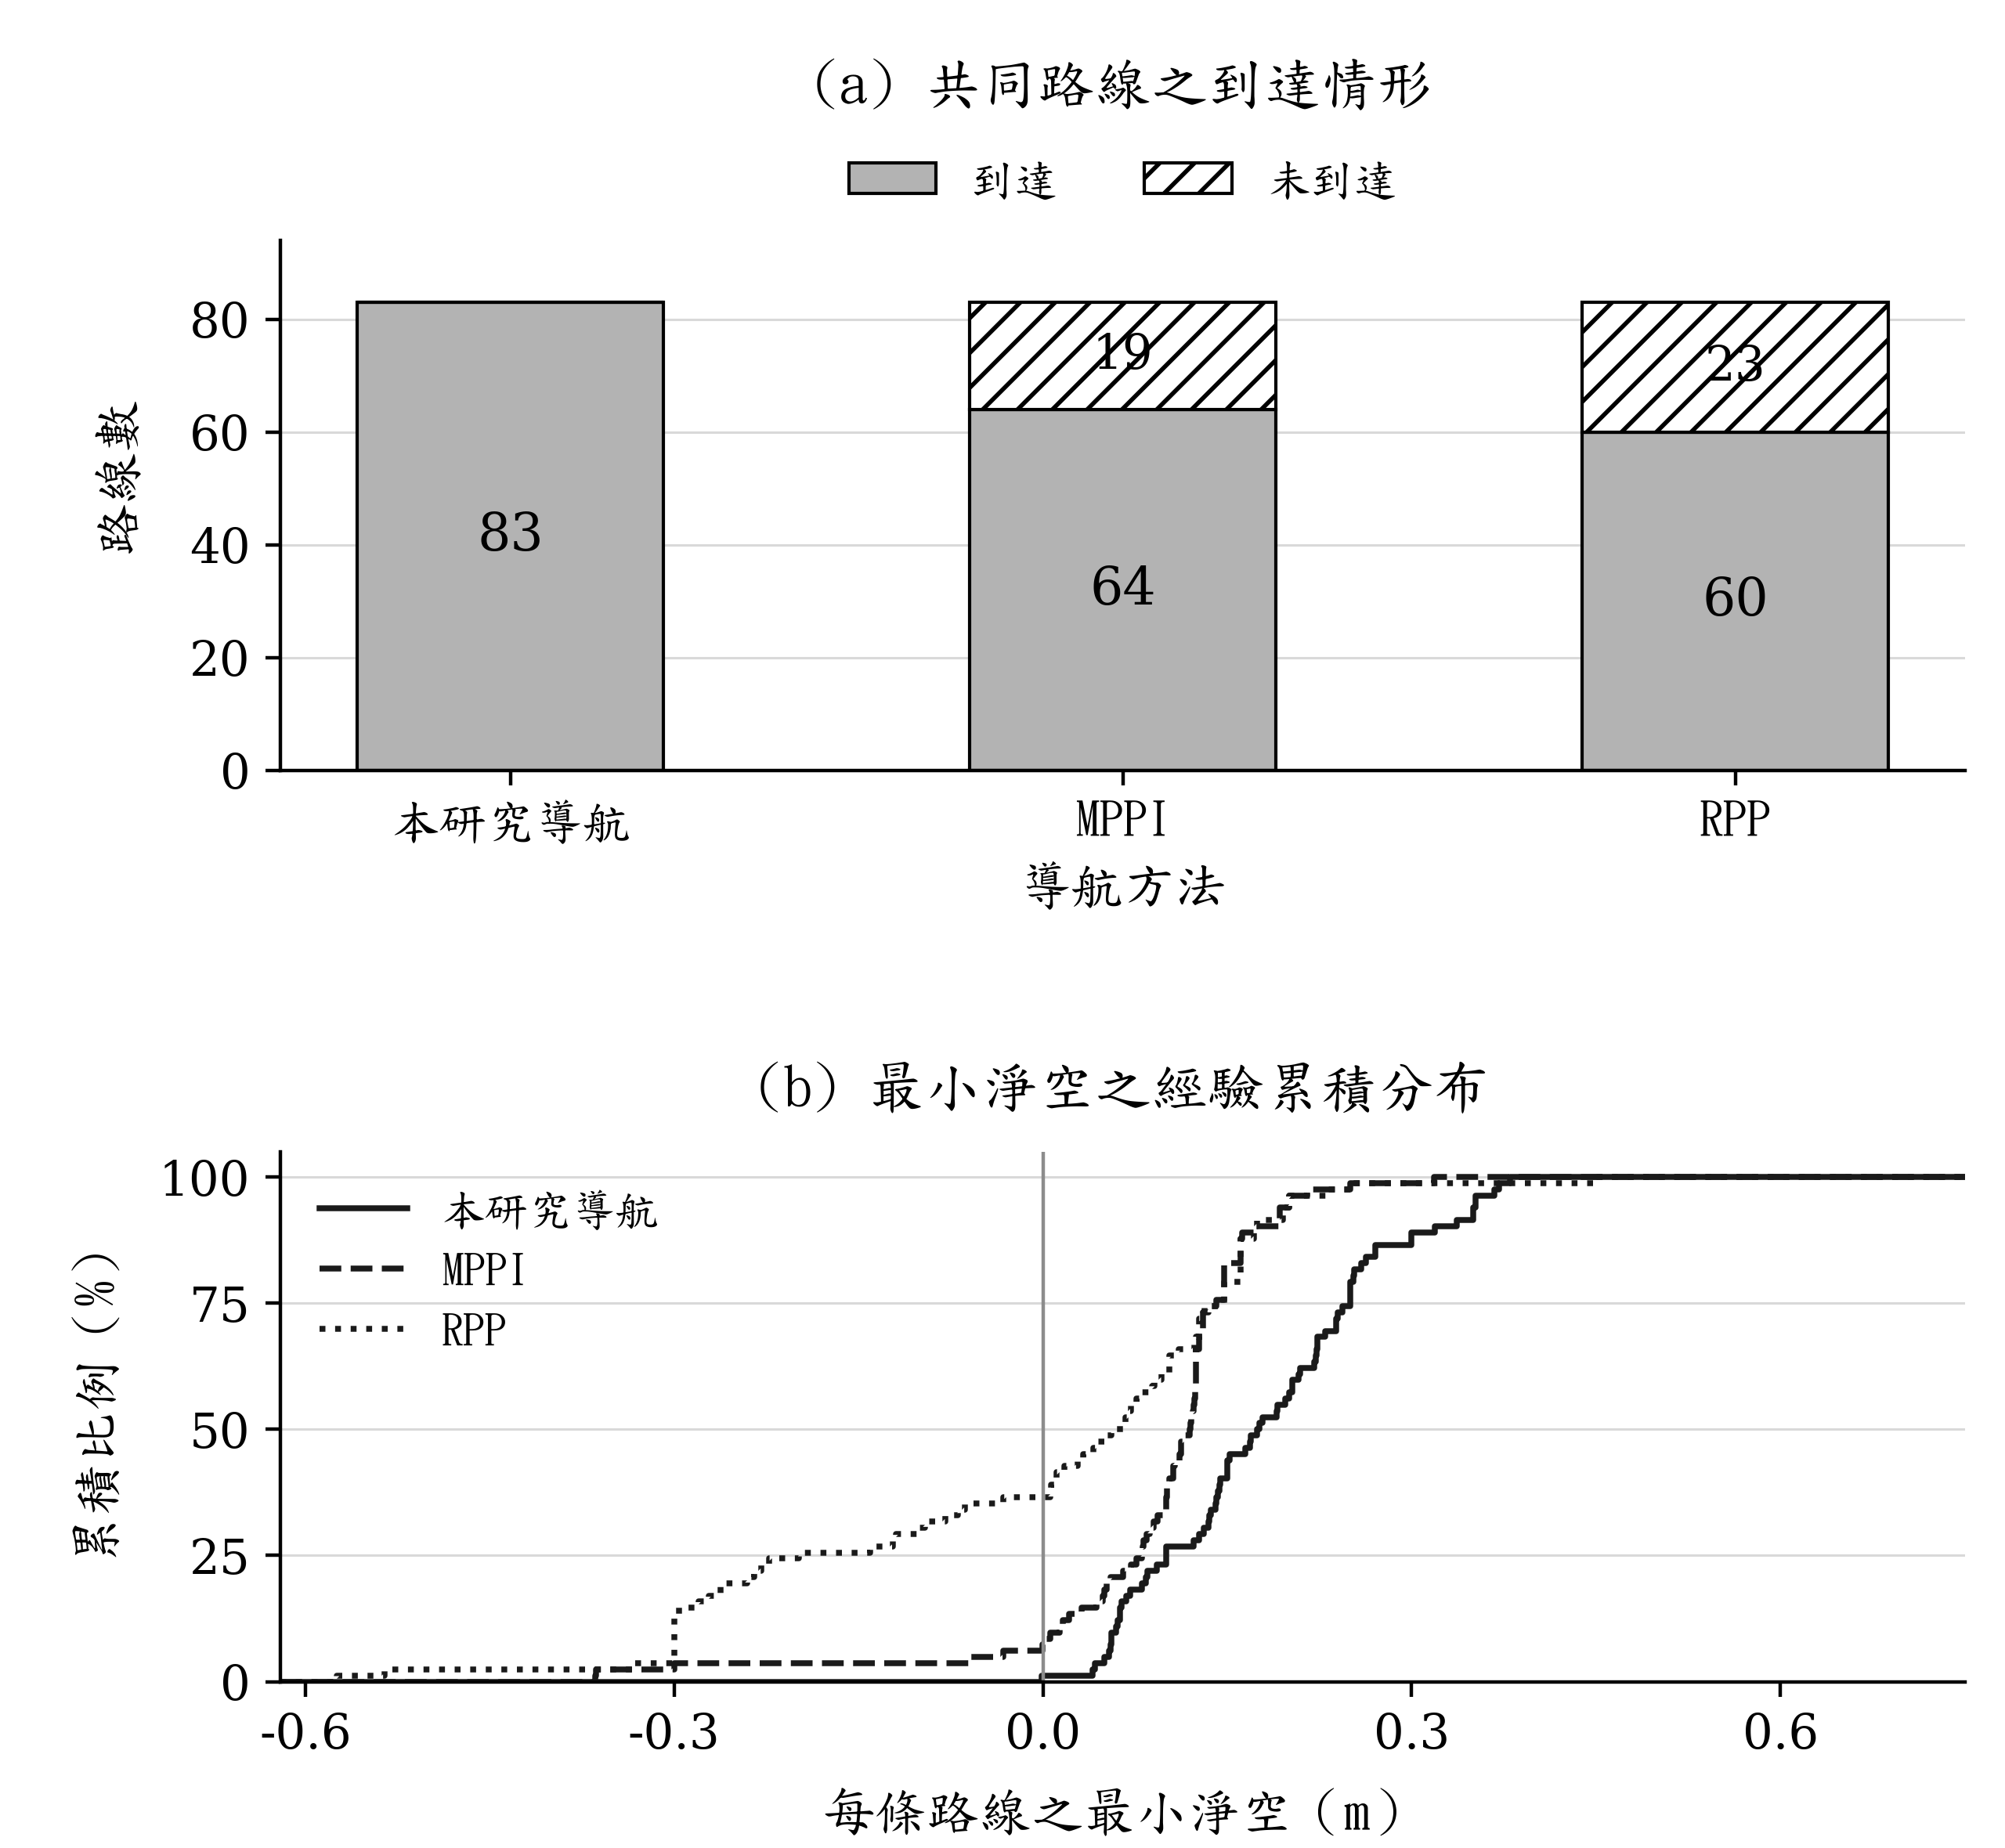
\includegraphics[width=0.98\textwidth]{figsrc/ch04/navigation_method_comparison.png}
    \caption{不同導航方法之到達與淨空比較：
    (a) $83$ 條共同路線的到達情形；
    (b) $82$ 條共同有效路線之最小淨空經驗累積分布。
    (b) 中零淨空左側對應評估外形曾出現幾何重疊的路線。}
    \label{fig:ch4_navigation_method_comparison}
\end{figure}

三者的到達時間中位數分別為 $102.6$、$48.6$ 與 $73.9$ s。
本研究導航配置需要較長時間完成通行，
其到達完整性與間距表現伴隨較高的時間成本。
由於各方法成功到達的路線集合不同，
時間中位數需與到達數量共同解讀；
較短時間可能同時反映較快行進與較困難路線未完成的選樣差異。

本研究導航配置將障礙相對運動納入 CBF，
並以原始掃描限制近距離接近速度；
MPPI 則依其取樣軌跡與代價地圖評分更新命令，
RPP 依前視路徑調整前進與轉向。
上述結果反映這些完整配置在本場景中的行為差異，
可用運動方向、預測時域與避障處理方式均屬比較條件的一部分。

% ==================================================
% 4.3.3 控制屏障與雷射防護之消融比較
% ==================================================
\subsection{控制屏障與雷射防護之消融比較}
\label{subsec:cbf_scan_shield_ablation}

為分析兩個避障層次的作用，
以相同 GMPC 路徑追蹤控制器建立四種配置：
A 為兩者皆關閉，B 僅啟用 CBF，
C 僅啟用原始雷射防護，D 則同時啟用兩者。
比較使用四種配置皆具有效結果的 $28$ 條共同路線，
並保留相同場景、起終點、速度上限與其餘控制設定。
四種配置在此集合中皆到達目標，
因此可在相同到達範圍下比較幾何重疊與時間成本。

\cref{tab:ch4_navigation_ablation}列出消融結果。
配置 A 的幾何重疊路線數為 $22$；
加入 CBF 後，配置 B 降至 $3$，
僅啟用雷射防護的配置 C 則為 $2$。
配置 D 在本次共同集合中未記錄到負淨空，
且全部路線中的最差淨空約為 $0.022$ m。
這些結果顯示，兩種模組各自啟用時均能減少幾何重疊，
共同啟用時則在本集合中取得較完整的通行結果。

\begin{table}[htbp]
    \centering
    \caption{CBF 與原始雷射防護之消融比較（共同 $28$ 條路線）}
    \label{tab:ch4_navigation_ablation}
    \begingroup
    \small
    \setlength{\tabcolsep}{4pt}
    \renewcommand{\arraystretch}{1.25}
    \begin{tabular}{c c c c c c}
        \hline
        配置 & CBF & 雷射防護
        & \shortstack{重疊\\路線數}
        & \shortstack{最小淨空\\中位數（m）}
        & \shortstack{到達時間\\中位數（s）} \\
        \hline
        A & 關 & 關 & $22$ & $-0.300$ & $79.2$  \\
        B & 開 & 關 & $3$  & $0.180$  & $98.0$  \\
        C & 關 & 開 & $2$  & $0.080$  & $88.4$  \\
        D & 開 & 開 & $0$  & $0.150$  & $104.3$ \\
        \hline
    \end{tabular}
    \endgroup
\end{table}

兩個模組作用於不同的資料與命令位置。
CBF 由追蹤後的障礙幾何與速度建立預測限制，
使避障需求直接參與控制輸入的求解；
原始雷射防護則在執行端處理有效回波，
限制最終命令沿近距離障礙方向的接近分量。
因此，兩者分別提供預測限制與執行端命令核對，
其組合效果可由 B、C 與 D 的差異觀察。

\cref{fig:ch4_navigation_ablation}(a)比較幾何重疊路線數，
(b)呈現相同路線集合下的到達時間分布。
配置 D 的時間中位數為 $104.3$ s，
高於配置 B 的 $98.0$ s 與配置 C 的 $88.4$ s。
其路徑長度中位數亦由配置 A 的約 $19.0$ m 增至 $21.8$ m，
反映此避障配置下較高的通行時間與路程成本。

\begin{figure}[htbp]
    \centering
    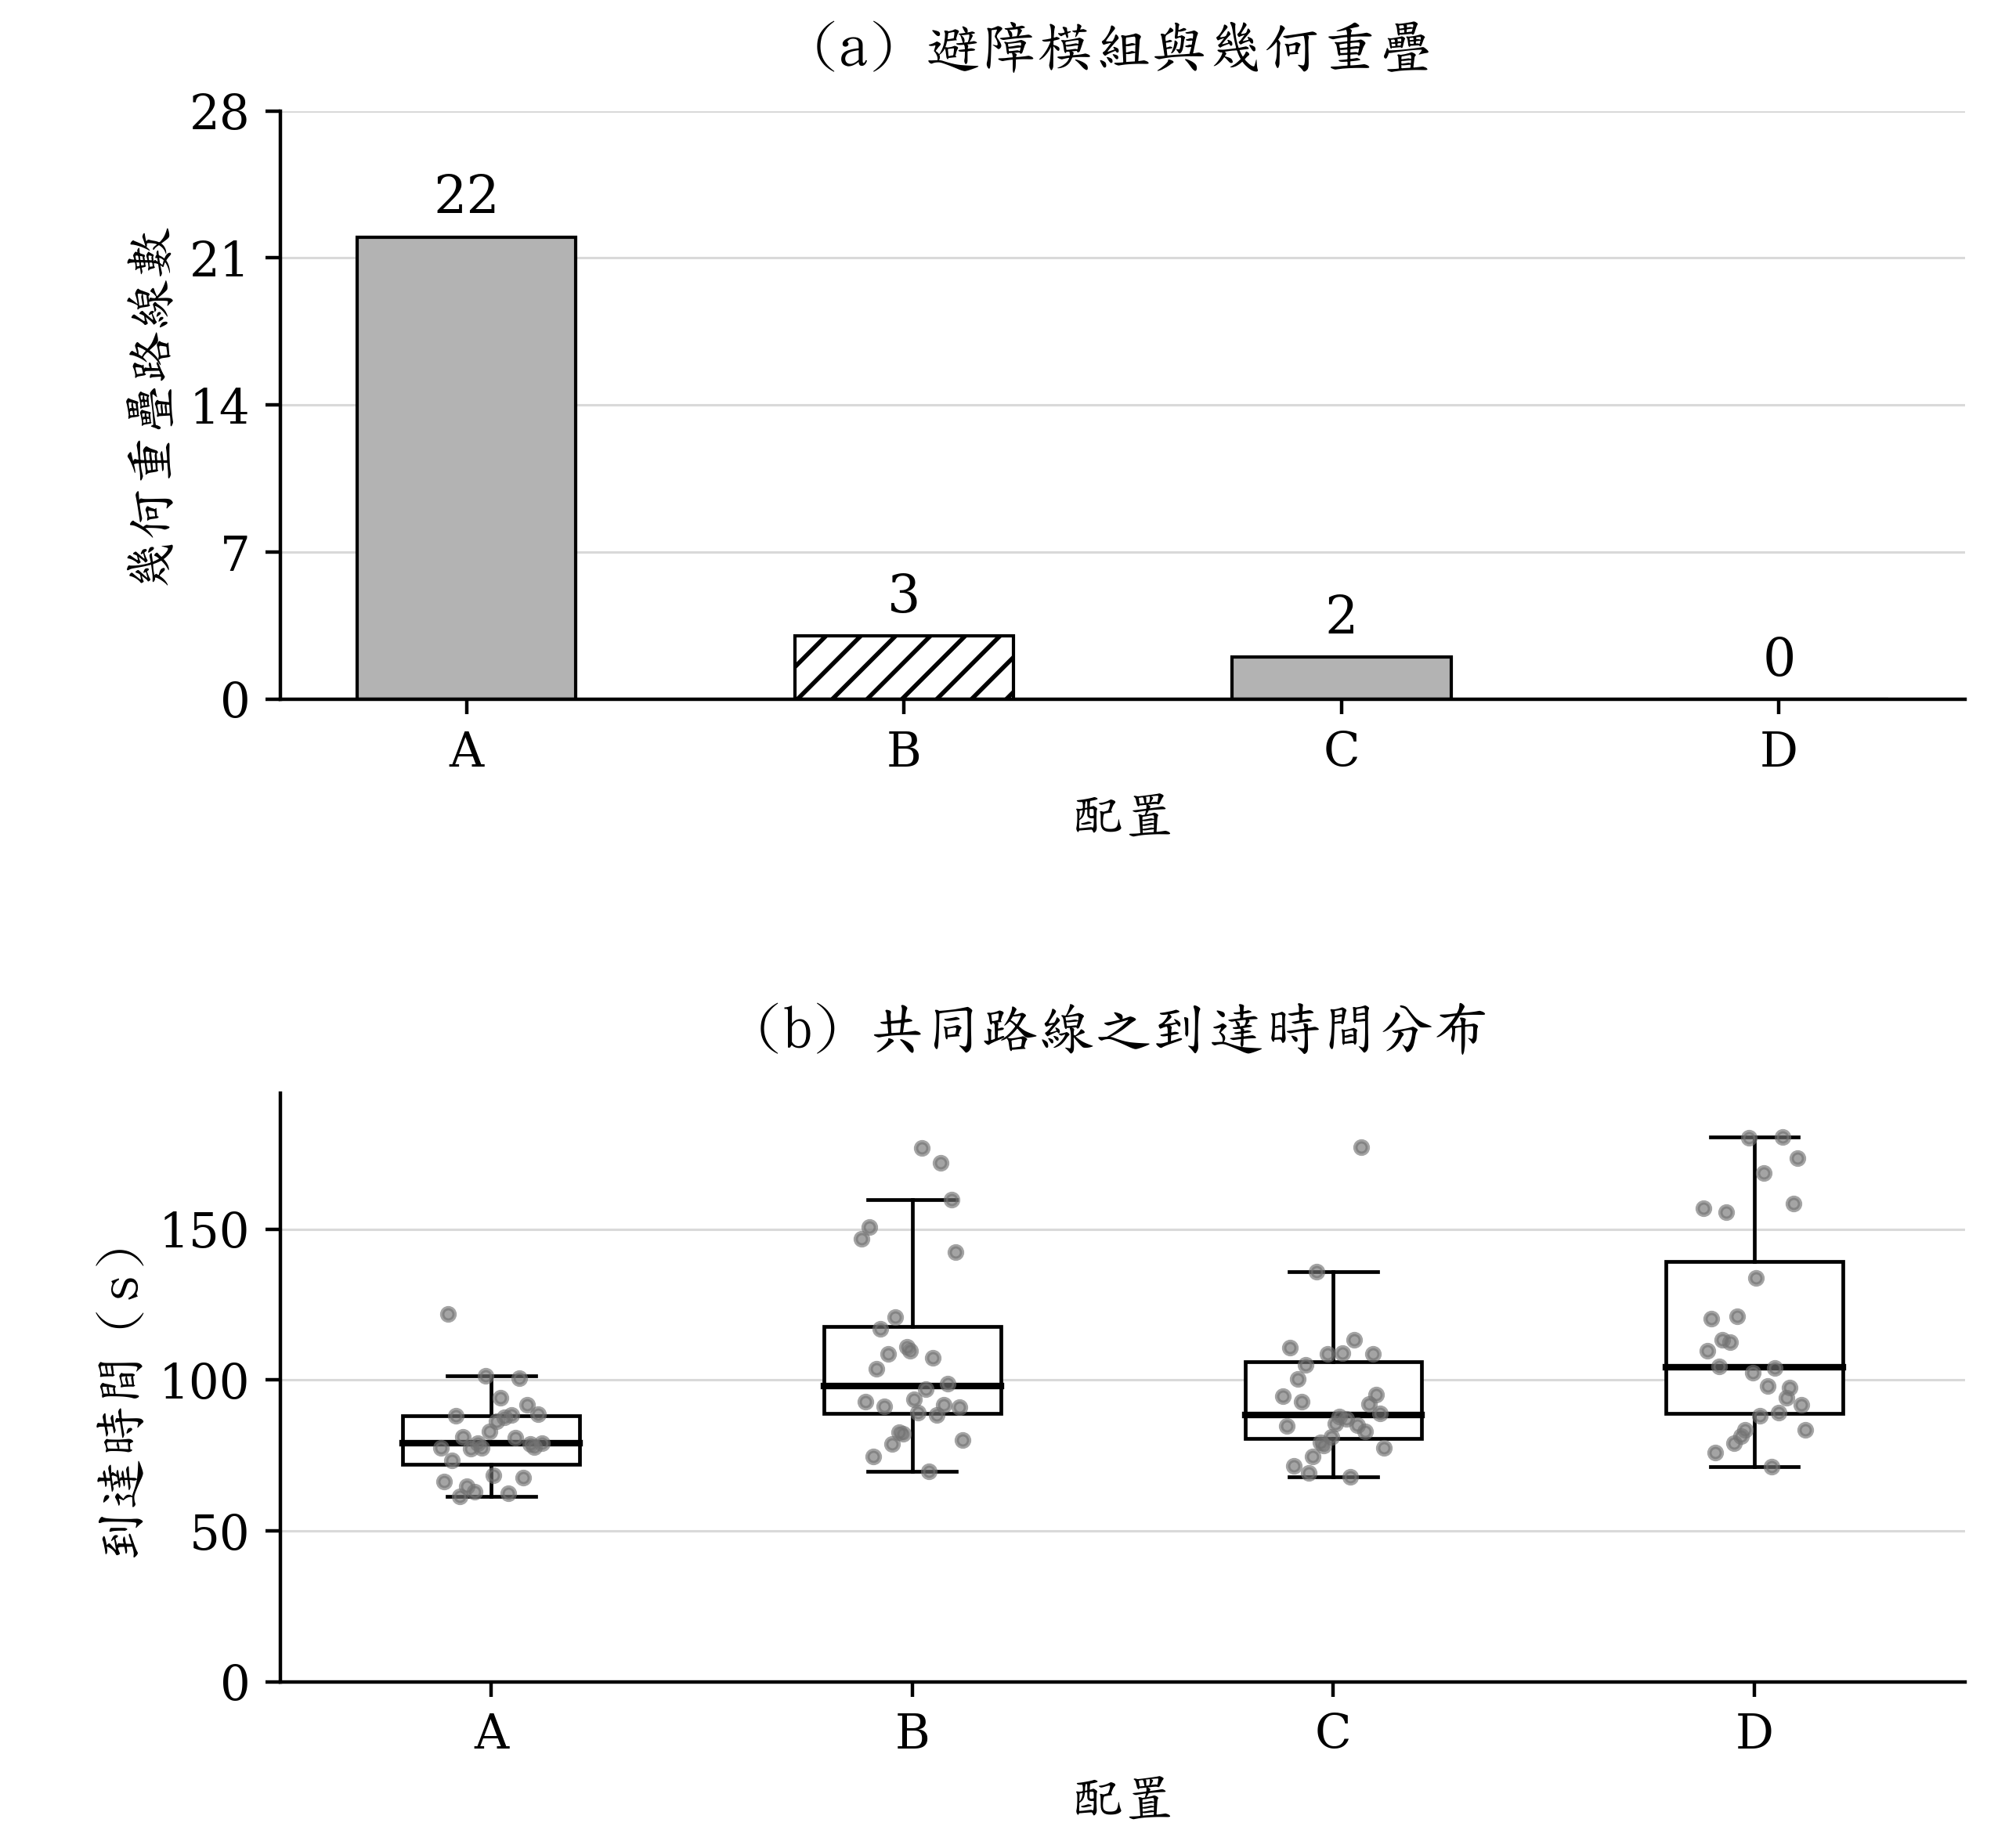
\includegraphics[width=0.98\textwidth]{figsrc/ch04/cbf_scan_shield_ablation.png}
    \caption{避障模組消融比較：
    (a) 共同路線中出現幾何重疊的路線數；
    (b) 到達時間分布，散點為各路線結果，箱體為第 $25$ 至 $75$ 百分位數，
    中線為中位數，鬚線為 $1.5$ 倍四分位距內的資料範圍。
    A 為兩者關閉，B 僅啟用 CBF，C 僅啟用雷射防護，D 為兩者啟用。}
    \label{fig:ch4_navigation_ablation}
\end{figure}

配置 B 的典型最小淨空高於配置 D，
但仍保有負淨空路線，說明單一中位數無法涵蓋全部交會情形。
同時檢查到達、重疊路線、最差淨空與時間分布，
可較完整地呈現避障配置的效果與代價。
本組結果支持在所測場景與速度範圍下保留兩層防護，
並於後續全身操作中持續核對其命令作用與任務銜接。
